\Askhsh{16755_SOLUTION}{1}
\begin{ylh}{1}
    \item [Ομοιότητα τριγώνων]
\end{ylh}
\begin{wrapfigure}[22]{r}{5.5cm} % Adjust number of lines (22) and width as needed based on text flow
    \centering
    \begin{tikzpicture}[scale=0.8]
        % Define points C, B, D on the x-axis and A above
        \tkzDefPoint(0,0){C} % Point Gamma
        \tkzDefPoint(10,0){B} % Point B
        \tkzDefPoint(2.5,0){D} % Point Delta, based on the ratios AΓ = 2ΓΔ and BΓ = 2AΓ.
                              % If AΓ is set to a length (e.g., 5 units), then BΓ = 10 units and ΓΔ = 2.5 units.
        \tkzDefPoint(3,4){A} % Point A, chosen so that AΓ = sqrt(3^2 + 4^2) = 5 units.

        % Draw the segments forming the triangles
        \tkzDrawSegments(A,B B,C C,A A,D)

        % Label the points
        \tkzLabelPoint[below left](C){$\Gamma$}
        \tkzLabelPoint[below right](B){B}
        \tkzLabelPoint[below](D){$\Delta$}
        \tkzLabelPoint[above](A){A}

        % Draw points as small circles
        \tkzDrawPoints(A,B,C,D)
    \end{tikzpicture}
\end{wrapfigure}

ΛΥΣΗ

\begin{alist}
    \item Αφού δίνονται ότι $\text{B}\Gamma = 2\text{A}\Gamma$ και $\text{A}\Gamma = 2\Gamma\Delta$, θα είναι:
    \[
        \frac{\text{B}\Gamma}{\text{A}\Gamma} = 2 \quad \text{και} \quad \frac{\text{A}\Gamma}{\Gamma\Delta} = 2
    \]

    \item Τα τρίγωνα $\text{AB}\Gamma$ και $\Delta\text{A}\Gamma$ έχουν:
    \[
        \frac{\text{B}\Gamma}{\text{A}\Gamma} = 2
    \]
    \[
        \frac{\text{A}\Gamma}{\Gamma\Delta} = 2
    \]
    $\hat{\Gamma}$ (κοινή)

    Επομένως, τα τρίγωνα $\text{AB}\Gamma$ και $\Delta\text{A}\Gamma$ είναι όμοια, αφού έχουν δύο πλευρές ανάλογες μία προς μία και τις περιεχόμενες στις πλευρές αυτές γωνίες ίσες.

    Αφού τα τρίγωνα $\text{AB}\Gamma$ και $\Delta\text{A}\Gamma$ είναι όμοια, τότε θα έχουν ίσες τις γωνίες που βρίσκονται απέναντι από ομόλογες πλευρές τους. Επομένως, έχουμε:
    \begin{itemize}
        \item $\text{B}\hat{\text{A}}\Gamma = \Gamma\hat{\Delta}\text{A}$, αφού βρίσκονται απέναντι από τις πλευρές $\text{B}\Gamma$ και $\text{A}\Gamma$ αντίστοιχα.
        \item $\hat{\text{B}} = \Delta\hat{\text{A}}\Gamma$, αφού βρίσκονται απέναντι από τις πλευρές $\text{A}\Gamma$ και $\Gamma\Delta$ αντίστοιχα.
    \end{itemize}
\end{alist}